\section{Results}

\subsection{Evolutionary History}

% https://mybinder.org/v2/gh/mmore500/dishtiny/e17e6d5e258b7aacac72d44922008ab14e80e182?filepath=binder%2Fbucket%3Dprq49%2Fa%3Dall_stints_all_series_profiles%2Bendeavor%3D16%2Fcase_study_16005.ipynb
Due to the distributed nature of the experimental framework, we did not perform perfect phylogeny tracking.
However, we did track the total number of ancestors seeded into stint 0 with extant descendants.
At the end of stints 0 and 1, three distinct original phylogenetic roots were present in the population.
From stint 2 onward, only two distinct original phylogenetic roots were present.

% https://mybinder.org/v2/gh/mmore500/dishtiny/e17e6d5e258b7aacac72d44922008ab14e80e182?filepath=binder%2Fbucket%3Dprq49%2Fa%3Dall_stints_all_series_profiles%2Bendeavor%3D16%2Fcase_study_16005.ipynb
We performed follow-up analyses on specimens sampled from the lowest original phylogenetic root ID present in the population.
For the first two stints, this was root ID 2,378.
During stint 2, original phylogenetic root 2,378 went extinct.
So, all further follow-up analyses were sampled from descendants of ancestor 12,634.

We also tracked the number of genomes reconstituted at the outset of each stint with extant descendants at the end of that stint.
This count grows from approximately 10 around stint 15 to upwards of 30 around stint 40 (Supplementary Figure \ref{fig:phylogeny:stint_roots}\citep{Moreno_2021}).
Among descendants of the lowest original phylogenetic root, the number of independent lineages spanning a stint also increases from around 5 to around 15
(Supplementary Figure \ref{fig:phylogeny:lowestroot_stint_roots} \citep{Moreno_2021}).
This decrease in phylogenetic consolidation on a stint-by-stint basis correlates with the waning number of simulation updates performed per stint (Supplementary Figures \ref{fig:phylogeny:updates_vs_stint_roots} and \ref{fig:phylogeny:log_updates_vs_stint_roots} \citep{Moreno_2021}).
More complete phylogenetic data will be necessary in future experiments to address questions about the possibility of long-term stable coexistence beyond the two strains supported under the explicit     diversity maintenance scheme.

% https://mybinder.org/v2/gh/mmore500/dishtiny/e17e6d5e258b7aacac72d44922008ab14e80e182?filepath=binder%2Fbucket%3Dprq49%2Fa%3Dall_stints_all_series_profiles%2Bendeavor%3D16%2Fcase_study_16005.ipynb
On the specimen from stint 100 used in the final case study, an evolutionary history of 20,212 cell generations had elapsed.
Of these cellular reproductions, 11,713 (58\%) had full kin group commonality, 7,174 had partial kin group commonality (35\%), and 1,325 had no kin group commonality (7\%).
On this specimen, 1,672 mutation events had elapsed.
During these events, 7,240 insertion-deletion alterations had occurred and 26,153 point mutations had occurred.
This strain experienced a selection pressure of 18\% over its evolutionary history, meaning that only 82\% of the mutations that would be expected given the number of cellular reproductions that had elapsed were present. 

\subsection{Qualitative Morphological Categorizations}

% \pragmaonce

% adapted from https://www.overleaf.com/learn/latex/Commands
\providecommand{\dissertationelse}[2]{%
% adapted from https://tex.stackexchange.com/a/33577
\ifdefined\DISSERTATION
#1
\else
#2
\fi
}

% \pragmaonce

% adapted from https://www.overleaf.com/learn/latex/Commands
\providecommand{\dissertationexclude}[1]{%
% adapted from https://tex.stackexchange.com/a/33577
\ifdefined\DISSERTATION
\else
#1
\fi
}

% \pragmaonce

% adapted from https://www.overleaf.com/learn/latex/Commands
\providecommand{\dissertationonly}[1]{%
% adapted from https://tex.stackexchange.com/a/33577
\ifdefined\DISSERTATION%
#1%
\else%
\fi
}


\newcommand{\includesnapshot}[1] {%
\adjustbox{trim={0.05\width} {0.35\width} {0.05\width} {0.35\width},clip}%
    {\includegraphics[height=\dissertationexclude{0.3}\dissertationonly{0.25}\textheight]{#1}}
}
\newcommand{\morphtext}[1] {%
\color[HTML]{FFFFFF} \huge \raisebox{1.2em}{\textbf{#1}}%
}
\newcommand{\videolink}[1] {%
\raisebox{
\dissertationexclude{2.8em}
\dissertationonly{2.2em}
}{\begin{minipage}{\dissertationelse{2.4cm}{1.3 cm}} \dissertationelse{\fontsize{6}{7}\selectfont}{\tiny}\url{#1} \end{minipage}}
}
\newcommand{\descript}[1] {%
\raisebox{
  \dissertationexclude{2.8em}
  \dissertationonly{2.2em}
}{\begin{minipage}{\linewidth}\dissertationonly{\fontsize{8}{8}\selectfont} #1 \end{minipage}}
}


{
\catcode`\%=12
\begin{table*}
\begin{tabular}{cp{0.4\textwidth}ll}
\multicolumn{1}{l}{\textbf{ID}}               & \textbf{Morphology} & \textbf{Snapshot} & \textbf{Video} \\
\cellcolor[HTML]{4C72B0}{ \morphtext{a} } & \descript{Individual cells, no multicellular kin groups. Resource use is low---most cells simply hoard resource until their stockpile is beyond sufficient to reproduce. Only a handful of cells intermittently expend resource.} & \includesnapshot{\detokenize{snapshots/sanitized/a=kin-group-id+idx=0+proc=0+series=16005+stint=0+thread=0+update=28991+ext=.png}}             &  \videolink{https://hopth.ru/21/b=prq49+s=16005+t=0+v=video+w=specimen}          \\
\cellcolor[HTML]{DD8452}{\morphtext{b}} & \descript{Mostly individual cells, with some two-, three-, and four-cell groups evenly spread out. Resource usage occurs in short spurts in one or two adjacent cells. } & \includesnapshot{\detokenize{snapshots/sanitized/a=kin-group-id+idx=0+proc=0+series=16005+stint=1+thread=0+update=14271+ext=.png}}                 & \videolink{https://hopth.ru/21/b=prq49+s=16005+t=1+v=video+w=specimen}              \\
\cellcolor[HTML]{55A868}{\morphtext{c}} & \descript{Large multicellular groups dominate, consisting of hundreds of cells. Group growth is unchecked and continues until cells' resource stockpiles are entirely depleted by the excess group size penalty.} & \includesnapshot{\detokenize{snapshots/sanitized/a=kin-group-id+idx=0+proc=0+series=16005+stint=2+thread=0+update=17471+ext=.png}}                  & \videolink{https://hopth.ru/21/b=prq49+s=16005+t=2+v=video+w=specimen}             \\
\cellcolor[HTML]{C44E52}{\morphtext{d}} & \descript{Clear groups of 10 to 15 cells form. Cell proliferation appears somewhat more active at the periphery of groups compared to the interior.} & \includesnapshot{\detokenize{snapshots/sanitized/a=kin-group-id+idx=0+proc=0+series=16005+stint=14+thread=0+update=16959+ext=.png}}                  & \videolink{https://hopth.ru/21/b=prq49+s=16005+t=14+v=video+w=specimen}               \\
\cellcolor[HTML]{8172B3}{\morphtext{e}} & \descript{Groups are visibly elongated along the horizontal axis. After initial development, some gradual, irregular growth occurs along the vertical axis.} & \includesnapshot{\detokenize{snapshots/sanitized/a=kin-group-id+idx=0+proc=0+series=16005+stint=15+thread=0+update=16639+ext=.png}}                  & \videolink{https://hopth.ru/21/b=prq49+s=16005+t=15+v=video+w=specimen}              \\
\cellcolor[HTML]{937860}{\morphtext{f}} & \descript{Groups are horizontally elongated similarly to morphology $e$, but have a larger consistent vertical thickness of three or four cells.} & \includesnapshot{\detokenize{snapshots/sanitized/a=kin-group-id+idx=0+proc=0+series=16005+stint=39+thread=0+update=10303+ext=.png}}                  & \videolink{https://hopth.ru/21/b=prq49+s=16005+t=39+v=video+w=specimen}             \\
\cellcolor[HTML]{DA8BC3}{\morphtext{g}} & \descript{Initial group growth is almost entirely horizontal, with groups usually taking up only one row of cells. However, after an apparent timing cue groups perform a brief bout of aggressive vertical growth.} & \includesnapshot{\detokenize{snapshots/sanitized/a=kin-group-id+idx=0+proc=0+series=16005+stint=45+thread=0+update=12991+ext=.png}}                  & \videolink{https://hopth.ru/21/b=prq49+s=16005+t=45+v=video+w=specimen}              \\
\cellcolor[HTML]{8C8C8C}{\morphtext{h}} & \descript{Groups grow horizontally and then proliferate vertically on a timing cue like morph $e$. However, after that timing cue cell proliferation is incessant with almost no resource retention.} & \includesnapshot{\detokenize{snapshots/sanitized/a=kin-group-id+idx=0+proc=0+series=16005+stint=59+thread=0+update=11839+ext=.png}}                  & \videolink{https://hopth.ru/21/b=prq49+s=16005+t=59+v=video+w=specimen}              \\
\cellcolor[HTML]{CCB974}{\morphtext{i}} & \descript{Irregular groups of mostly less than ten cells. Incessant proliferation with almost no resource retention leads to rapid group turnover.} & \includesnapshot{\detokenize{snapshots/sanitized/a=kin-group-id+idx=0+proc=0+series=16005+stint=74+thread=0+update=12991+ext=.png}}                  & \videolink{https://hopth.ru/21/b=prq49+s=16005+t=74+v=video+w=specimen}              \\
\cellcolor[HTML]{64B5CD}{\morphtext{j}} & \descript{
Groups grow horizontally and then proliferate vertically on a timing cue like morph $e$. However, several viable horizontal-bar offspring groups form before forced fragmentation.} & \includesnapshot{\detokenize{snapshots/sanitized/a=kin-group-id+idx=0+proc=0+series=16005+stint=100+thread=0+update=8767+ext=.png}}                  & \videolink{https://hopth.ru/21/b=prq49+s=16005+t=100+v=video+w=specimen}
\end{tabular}

\caption{
\textbf{Qualitative morph phenotype categorizations.}
\footnotesize
Color coding of morph IDs has no significance beyond guiding the eye in scatter plots where points are labeled by morph.
Snapshot visualizes spatial layout of kin groups on toroidal grid at a fixed point in time.
Each cell corresponds to a small square tile.
Color hue denotes, and black borders divide, outermost kin groups; color saturation denotes, and white borders divide, innermost kin groups.
}
\label{tab:morph_descriptions}

\end{table*}
}


We performed a qualitative survey of the evolved life histories along the evolutionary timeline by analyzing video recordings of monocultures of each stint's representative specimen.

Table \ref{tab:morph_descriptions} summarizes the ten morphological categories we grouped specimens into.
In brief, specimens from early stints largely grew as unicellular or small multicellular groups (morphs $a$, $b$).
Then, the specimen from stint 14 grew as larger, symmetrical groups (morph $d$).
At stint 15, a distinct, asymmetrical horizontal bar morphology evolved (morph $e$).
%todo structure above is confusing
% Consistently left/right, indicating that somehow broke symmetrical of the simulation.
At stint 45, a delayed secondary spurt of group growth in the vertical direction arose (morph $g$).
This morphology was sampled frequently until stint 60 when morph $e$ began to be sampled primarily again.
However, morph $g$ was observed as late as stint 90.

Table \ref{tab:morph_descriptions} provides more detailed descriptions of each qualitative morph category as well as video and a still image example of each.
Supplementary Table \ref{tab:morph_by_stint} provides morph categorization for each stint as well as links to view the stint's specimen in a video or in-browser web simulation \citep{Moreno_2021}.

% \subsection{Multicellular Phenotypic Traits}

% In order for a transition in individuality, cells have to diminish their own immediate reproductive interests in order to prioritize the interests of the collective.
% In previous work with an earlier version of the system, we've seen multicellular traits evolve such as (blah from abstract) %todo
% \citep{moreno2021exploring}.

% The formation of kin group morphologies in this system does not necessarily imply a transition in individuality. 
% It is necessary to test to see if cells within groups are meaningfully cooperating.

% Because cell reproduction is necessarily adversarial in this system, we can test to see whether cells preferentially target or spare their group members.
% A conflict ratio of less than 1 implies that cells preferentially spare their members.
% We observed a  0.5 most of the time.

% Supplementary Figure \ref{fig:conflict:exactly_one} shows the  . %todo
% Supplementary Figure \ref{fig:conflict:at_least_one}
% Supplementary Figure \ref{fig:conflict:exactly_two}.
% However, could be an artifact of cell-offspring cooperation. 

% Interestingly, this strain appears to be using ``Is Child Cell Of,'' ``Is Parent Cell Of,'' ``Is Child Group Of,'' and the raw kin group ID of neighbors (but not the raw kin group ID of self).

% %todo change wording, not sure what you're hoping to say with first phrase
% To more conclusively, in future work we plan to look at the reproductive output at the interior of multicellular groups to see if these cells diminish their own reproductive output and to control for cellular relatedness when calculating this element of group cooperation. 

% We analyzed other traits characteristic of multicellularity, as well.

% We did not see widespread resource sharing over the evolutionary history.
% Only tiny fractions of cells, less than 1\%, appeared to share tiny amounts of the resource, less than 1\% of the resource required to reproduce per update (Supplementary Figures \ref{fig:resource_sharing:fraction_sharing_monoculture} and \ref{fig:resource_sharing:sharing_amount_monoculture}).
% However, in ten strains sampled along the evolutionary lineage, context-dependent resource-sending behavior contributed to fitness (Supplementary Figure \ref{fig:writable_perturbation}).
% Interestingly, another strain present in the population that was not the subject of analysis appeared to evolve widespread, higher-throughput resource sharing after stint 60 (Supplementary Figures \ref{fig:resource_sharing:fraction_sharing_evolve} and \ref{fig:resource_sharing:sharing_amount_evolve}).

% We observed widespread apoptosis over the evolutionary history.
% As shown in Supplementary Figure \ref{fig:apoptosis:apoptosis_stint}, in most monocultured representative strains, between 10 and 30\% of cell deaths were due to apoptosis.
% However, it is not clear if this apoptosis returned a fitness benefit.
% No context-dependent apoptosis behavior contributed to fitness for any sampled strain over the evolutionary history (Supplementary Figure \ref{fig:writable_perturbation}).
% It is unclear whether context-independent apoptosis might have a fitness benefit.

% The behavior seems like cells from within a group don't explicitly recognize one another according to group membership. However, they do recognize their cell parent/child and arrange themselves in a somewhat linear fashion that minimizes the potential for conflict between cells.
% Overall, there are elements of cooperation but is unclear to what extent this particular strain constitutes a proper fraternal transition in individuality.

\subsection{Fitness}

\begin{figure}

\begin{subfigure}{0.5\textwidth}

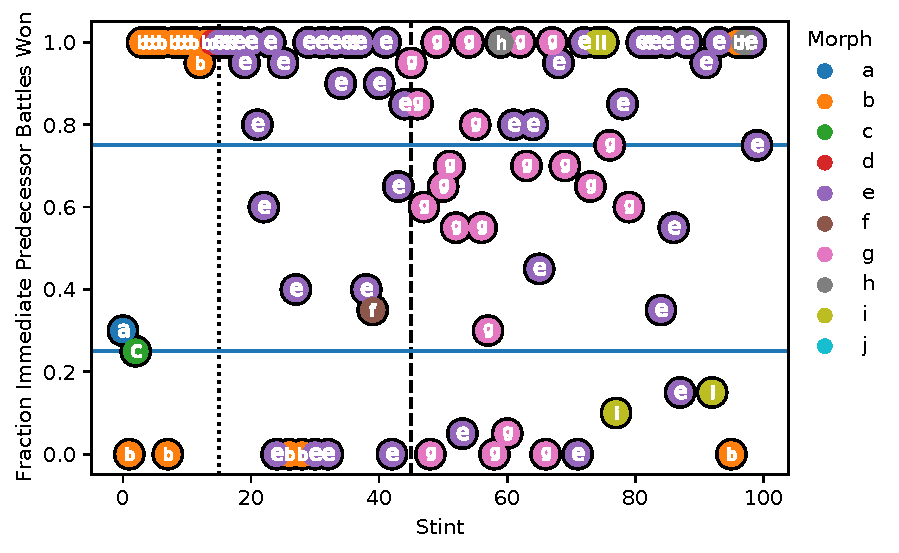
\includegraphics[width=\linewidth]{{plots/fitness/bucket=prq49+cat=morph+endeavor=16+transform=filter-Series-16005+viz=letterscatter-vline-binomialh0+x=stint+y=fraction-immediate-predecessor-battles-won+ext=}}

\caption{
Fraction of 20 independent competitions that were won against immediate predecessor population.
Blue horiziontal lines represent significance level $p < 0.05$ for binomial null hypothesis.
Neutral outcomes fall inside the blue bars, significant fitness increases fall above them, and significant fitness decreases fall below them.
}
\label{fig:fitness:fitness_neutrality}

\end{subfigure}%

\begin{subfigure}{0.5\textwidth}

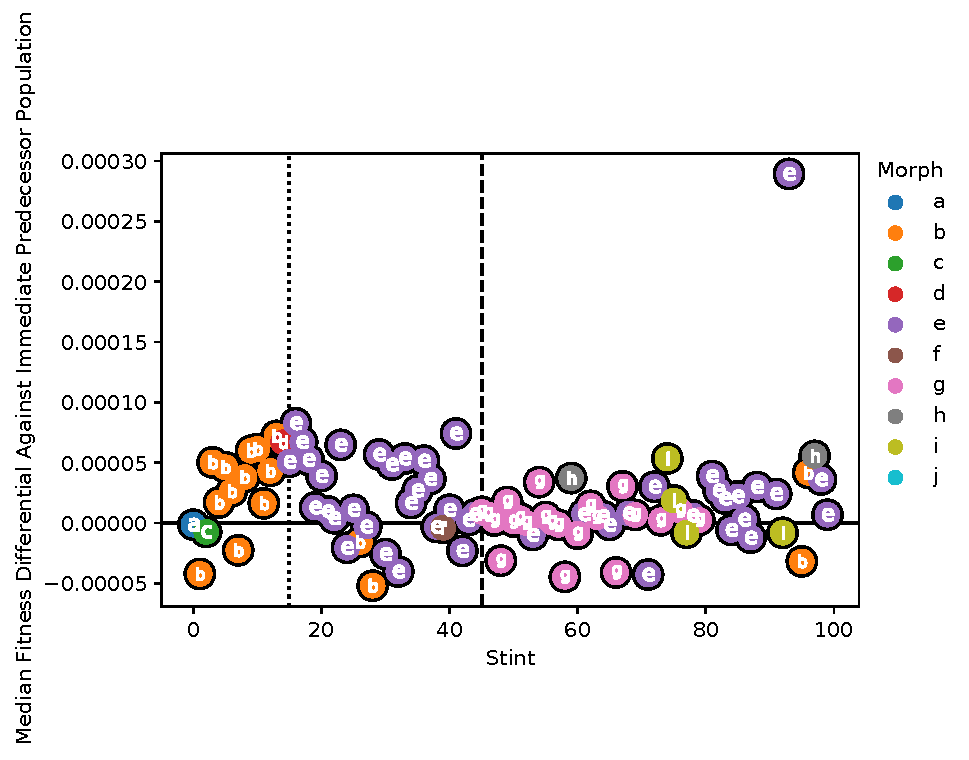
\includegraphics[width=\linewidth]{{plots/fitness/bucket=prq49+cat=morph+endeavor=16+transform=filter-Series-16005+viz=letterscatter-vline-hline+x=stint+y=median-fitness-differential-against-immediate-predecessor-population+ext=}}

\caption{Magnitude of fitness differential against immediately-preceding stint population.
Positive fitness differential indicates greater fitness compared to predecessor.
Solid horizontal line indicates neutral fitness differential.
}
\label{fig:fitness:fitness_magnitude}

\end{subfigure}%

\begin{subfigure}{0.5\textwidth}

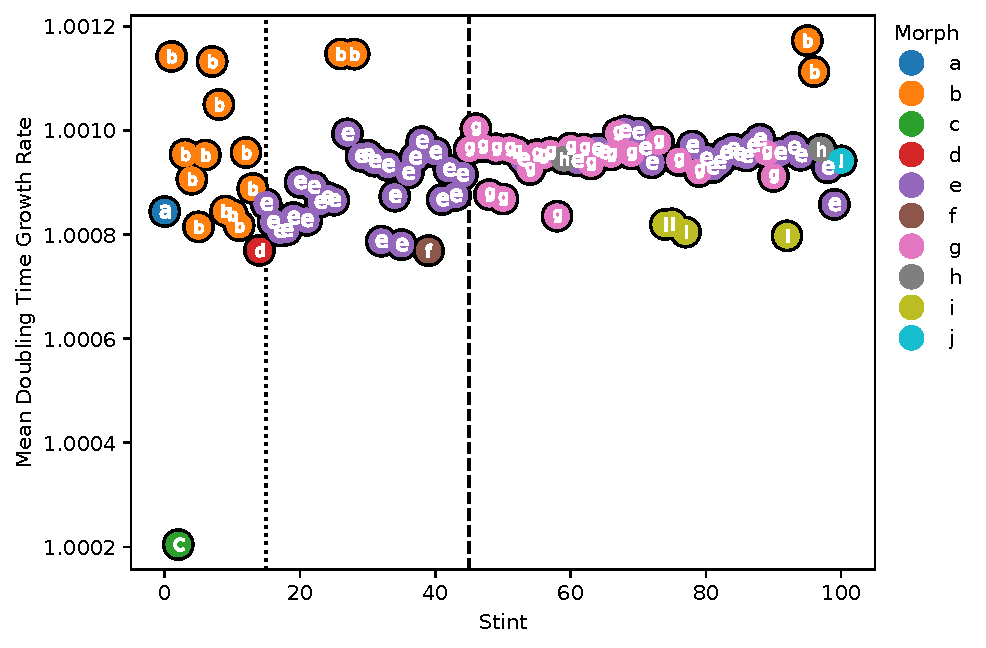
\includegraphics[width=\linewidth]{{plots/fitness/bucket=prq49+cat=morph+endeavor=16+transform=filter-Series-16005+viz=letterscatter-vline+x=stint+y=mean-doubling-time-growth-rate+ext=}}

\caption{Growth rate estimated from doubling time experiments, measuring time for a monoculture to grow from 0.25 maximum population size to 0.5 maximum population size.}
\label{fig:fitness:doubling_time}

\end{subfigure}%


\caption{ Fitness assays.
Color coding and letters correspond to qualitative morph codes described in Table \ref{tab:morph_descriptions}.
Dotted vertical line denotes emergence of morph $e$.
Dashed vertical line denotes emergence of morph $g$. }
\label{fig:fitness}

\end{figure}

In order to assess ongoing changes in fitness, we performed 20 replicate fitness competitions between the population seeded into each stint and the immediately population preceding it one stint prior.
We determined that a significant change in fitness had occurred between populations if one population won more than 15 of those competitions, corresponding to a significance level of $p < 0.05$ under the binomial null hypothesis.
Figure \ref{fig:fitness:fitness_neutrality} shows the fraction of competitions each stint won against its competitor.
Significant increases in fitness occur throughout the evolutionary history of the case study, but not at every stint.
In fact, some 20 stints exhibit significantly \textit{worse} fitness compared to their predecessor.
These episodes of population-wide fitness decline merit further inquiry, but seem likely to be related to the implicit, contextual nature of fitness in this system.

Figure \ref{fig:fitness:fitness_magnitude} shows the magnitude the median fitness differential observed for each predecessor competition.
Although the emergence of morphologies $d$, $e$, and $g$ were associated with significant increases in fitness, the magnitude of these fitness differentials is very similar to those of other stints (Figure \ref{fig:fitness:fitness_magnitude}).

We also measured growth rate of specimen strains by tracking doubling time (in updates) when seeded into quarter-full toroidal grids (Figure \ref{fig:fitness:doubling_time}).
Morph $b$ exhibited a fast growth rate early on that was never matched by later morphs.
This measure appears to be a poor overall proxy for fitness, highlighting the importance of biotic aspects of the simulation environment (which are not present in the empty space the assayed cells double into).

\subsection{Fitness Complexity}

\begin{figure}

\begin{subfigure}{0.5\textwidth}

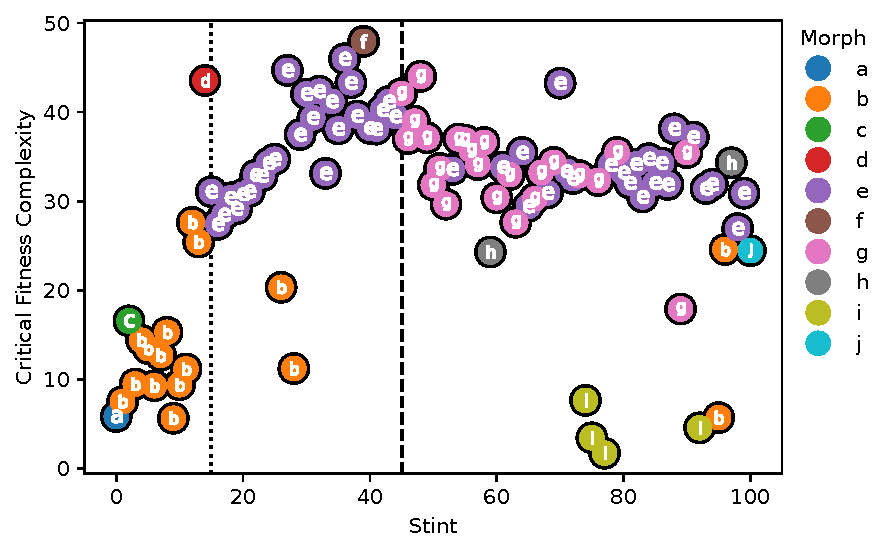
\includegraphics[width=\linewidth]{{plots/critical_fitness_complexity/bucket=prq49+cat=morph+endeavor=16+transform=filter-Series-16005+viz=letterscatter-vline+x=stint+y=critical-fitness-complexity+ext=}}

\caption{
Critical fitness complexity.
Number of single-site nopouts that significantly decrease fitness, adjusted for expected false positives.
}
\label{fig:fitness_complexity:critical_fitness_complexity}

\end{subfigure}%
% \begin{subfigure}{0.5\textwidth}

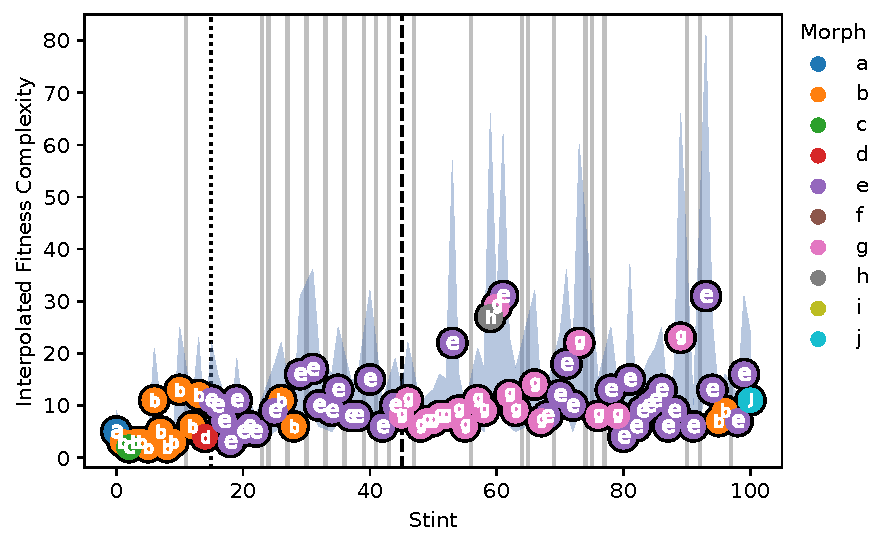
\includegraphics[width=\linewidth]{{plots/interpolated_fitness_complexity/bucket=prq49+cat=morph+endeavor=16+transform=filter-Series-16005+viz=letterscatter-err-vline+x=stint+y=interpolated-fitness-complexity+ext=.pdf}}

\caption{Interpolated fitness complexity.
Estimated number of non-critical sites that contribute to fitness.
Vertical gray lines represent stints with missing estimates due to bad phenotype-neutral nopouts.
Shaded areas represent 95\% confidence intervals.
Supplementary Figure \ref{fig:fitness_complexity_alt:interpolated_fitness_complexity_alt} shows the same data with smaller markers.
}
\label{fig:fitness_complexity:interpolated_fitness_complexity}

\end{subfigure}%
% \begin{subfigure}{0.5\textwidth}

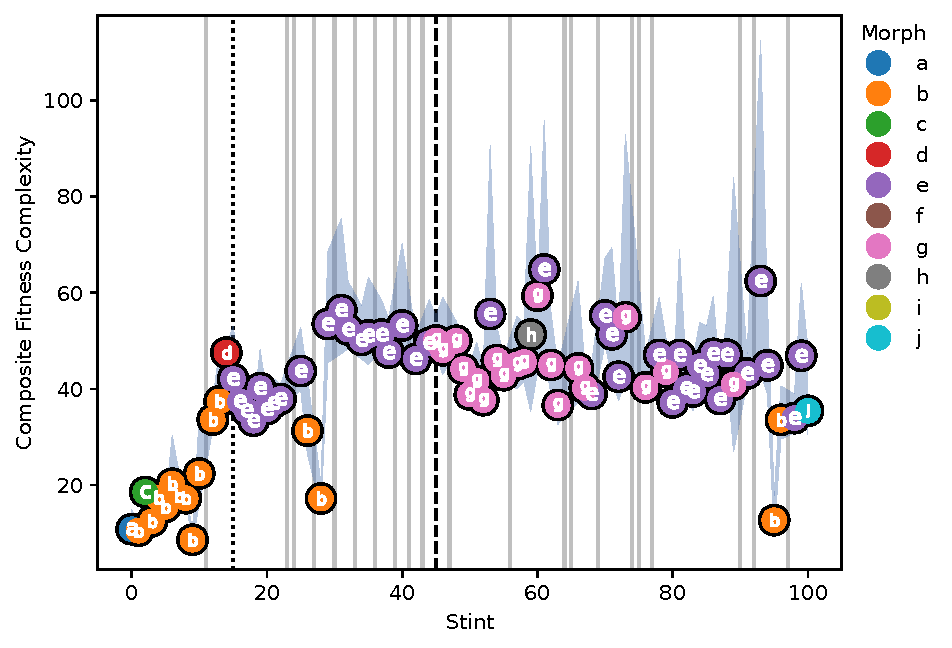
\includegraphics[width=\linewidth]{{plots/composite_fitness_complexity/bucket=prq49+cat=morph+ci=95+endeavor=16+transform=filter-Series-16005+viz=letterscatter-err-vline+x=stint+y=composite-fitness-complexity+ext=}}

\caption{
Composite fitness complexity.
Sum of critical fitness complexity and interpolated fitness complexity.
Error bars represent 95\% credible interval.
Vertical gray bars represent missing estimates due to bad phenotype-neutral nopouts.
Supplementary Figure \ref{fig:fitness_complexity_alt:composite_fitness_complexity_alt} shows the same data with smaller markers.
}
\label{fig:fitness_complexity:composite_fitness_complexity}

\end{subfigure}%

\caption{ Fitness complexity estimates. Color coding and letters correspond to qualitative morph codes described in Table \ref{tab:morph_descriptions}. 
Dotted vertical line denotes emergence of morph $e$.
Dashed vertical line denotes emergence of morph $g$.
}
\label{fig:fitness_complexity}

\end{figure}

Figure \ref{fig:fitness_complexity:critical_fitness_complexity} plots critical fitness complexity of specimens drawn from across the case study's evolutionary history.

Critical fitness complexity reaches more than 20 under morph $b$, jumps to more than 40 under morph $d$, drops to slightly more than 30 for morph $e$.
Critical fitness complexity reaches a peak of 48 sites around stint 39 then levels out and decreases.
% The evolution of morph $g$ is not associated with a clear change in critical fitness complexity.

% Interpolated fitness complexity remains much more steady over the course of evolutionary history, although the certainty of our estimate of interpolated fitness complexity varies greatly.
% Figure \ref{fig:fitness_complexity:interpolated_fitness_complexity} shows this.
% Sometimes we were not able to estimate composite fitness complexity because the phenotype neutral nopout was not truly neutral --- it was significantly less fit than wildtype.

% Figure \ref{fig:fitness_complexity:composite_fitness_complexity} shows composite fitness complexity, the sum of interpolated fitness complexity and critical fitness complexity.
% The highest best estimate of composite fitness complexity was 64 sites at stint 61.
% The highest lower bound estimate of composite fitness complexity was 49 sites at stint 70.

\subsection{Interface Complexity}

% \pragmaonce

% adapted from https://www.overleaf.com/learn/latex/Commands
\providecommand{\dissertationonly}[1]{%
% adapted from https://tex.stackexchange.com/a/33577
\ifdefined\DISSERTATION%
#1%
\else%
\fi
}

\begin{figure*}
\dissertationonly{\captionsetup[subfigure]{font=scriptsize}}
\dissertationonly{\captionsetup{font=footnotesize}}
\begin{subfigure}[t]{0.49\textwidth}

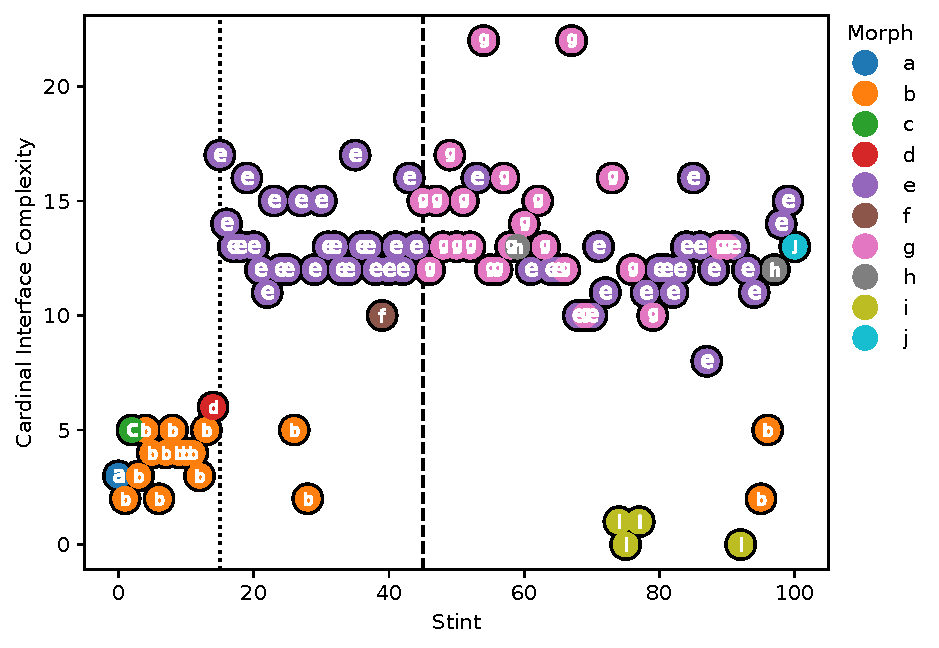
\includegraphics[width=\linewidth]{{plots/cardinal_interface_complexity/bucket=prq49+cat=morph+endeavor=16+transform=filter-Series-16005+viz=letterscatter+x=stint+y=cardinal-interface-complexity+ext=}}

\caption{Cardinal processor interface complexity, the total number of distinct interactions between a virtual CPU controlling cell behavior and its surroundings that contribute to fitness.
(Sum of Figures \labelcref{fig:interface_complexity:extrospective_interface_complexity,fig:interface_complexity:introspective_interface_complexity,fig:interface_complexity:writable_interface_complexity,fig:interface_complexity:intermessage_interface_complexity,fig:interface_complexity:intramessage_interface_complexity}.)}
\label{fig:interface_complexity:cardinal_interface_complexity}

\end{subfigure}%

\begin{subfigure}[t]{0.49\textwidth}

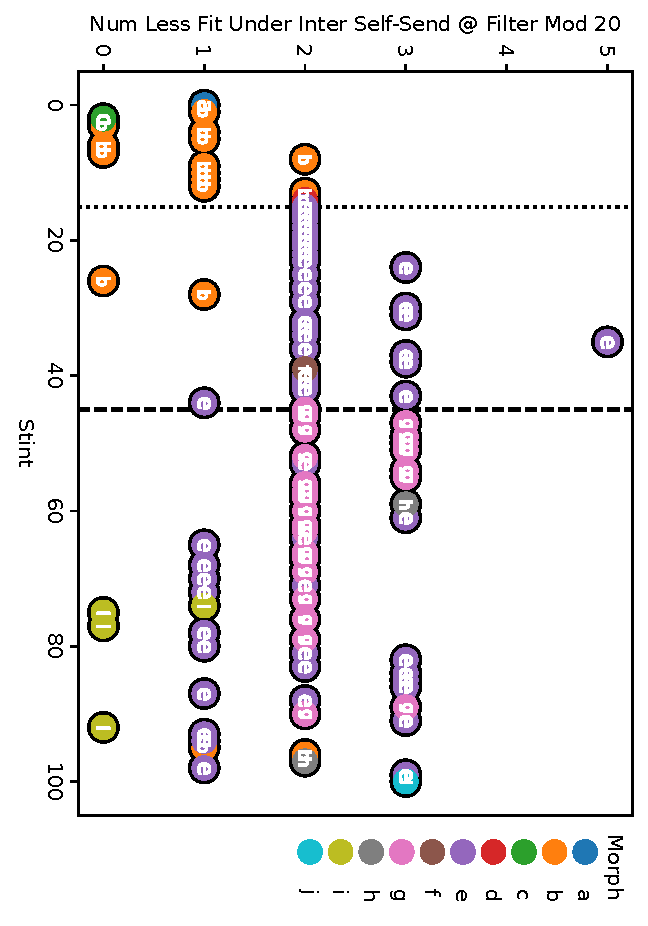
\includegraphics[width=\linewidth]{{plots/intermessage_interface_complexity/bucket=prq49+cat=morph+endeavor=16+transform=filter-Series-16005+viz=letterscatter-vline+x=stint+y=num-less-fit-under-inter-self-send-filter-mod-20+ext=}}

\caption{Intermessage interface complexity, the number of distinct inter-cell messages that contribute to fitness.}
\label{fig:interface_complexity:intermessage_interface_complexity}

\end{subfigure}%

\begin{subfigure}{0.5\textwidth}

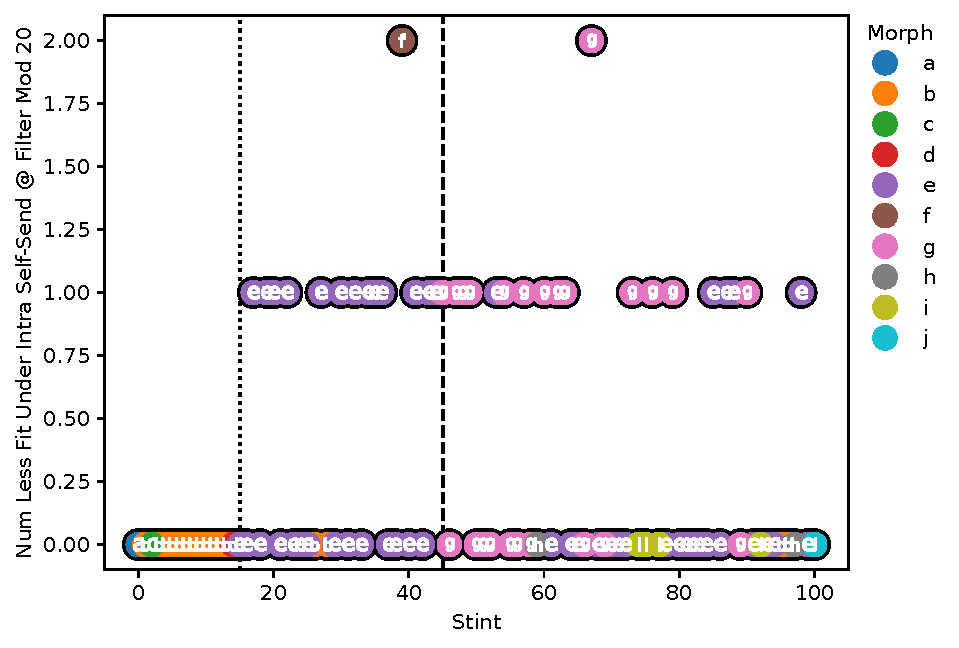
\includegraphics[width=\linewidth]{{plots/intramessage_interface_complexity/bucket=prq49+cat=morph+endeavor=16+transform=filter-Series-16005+viz=letterscatter-vline+x=stint+y=num-less-fit-under-intra-self-send-filter-mod-20+ext=}}

\caption{Intramessage interface complexity, the number of distinct inter-cell messages that contribute to fitness.}
\label{fig:interface_complexity:intramessage_interface_complexity}

\end{subfigure}%
\begin{subfigure}[t]{0.49\textwidth}

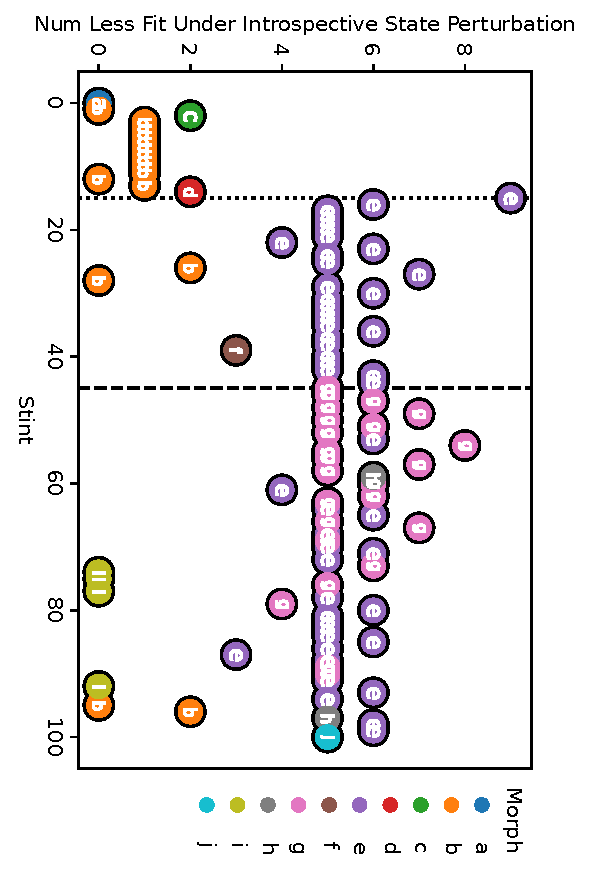
\includegraphics[width=\linewidth]{{plots/introspective_interface_complexity/bucket=prq49+cat=morph+endeavor=16+transform=filter-Series-16005+viz=letterscatter-vline+x=stint+y=num-less-fit-under-introspective-state-perturbation+ext=}}

\caption{Introspective interface complexity, the number of states viewed in the own cell that contribute to fitness. See Supplementary Figure \ref{fig:introspective_perturbation} for detail on the introspective states that contribute to fitness.}
\label{fig:interface_complexity:introspective_interface_complexity}

\end{subfigure}%

\begin{subfigure}{0.5\textwidth}

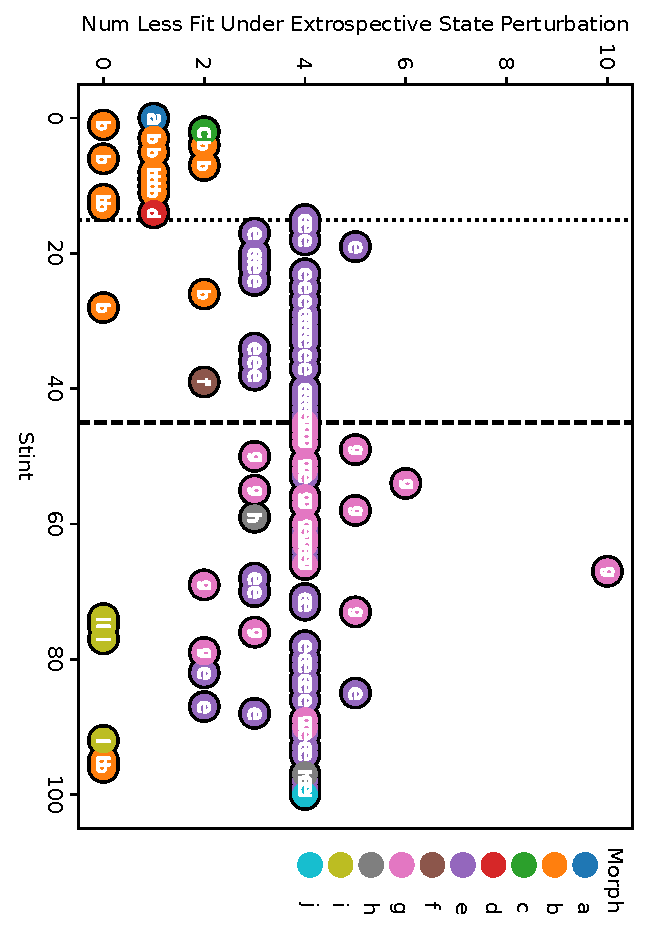
\includegraphics[width=\linewidth]{{plots/extrospective_interface_complexity/bucket=prq49+cat=morph+endeavor=16+transform=filter-Series-16005+viz=letterscatter-vline+x=stint+y=num-less-fit-under-extrospective-state-perturbation+ext=}}

\caption{ Extrospective interface complexity, the number of states viewed in neighboring cells that contribute to fitness.
See Supplementary Figure \ref{fig:extrospective_perturbation} for detail on the extrospective states that contribute to fitness. 
}
\label{fig:interface_complexity:extrospective_interface_complexity}

\end{subfigure}%
\begin{subfigure}{0.5\textwidth}

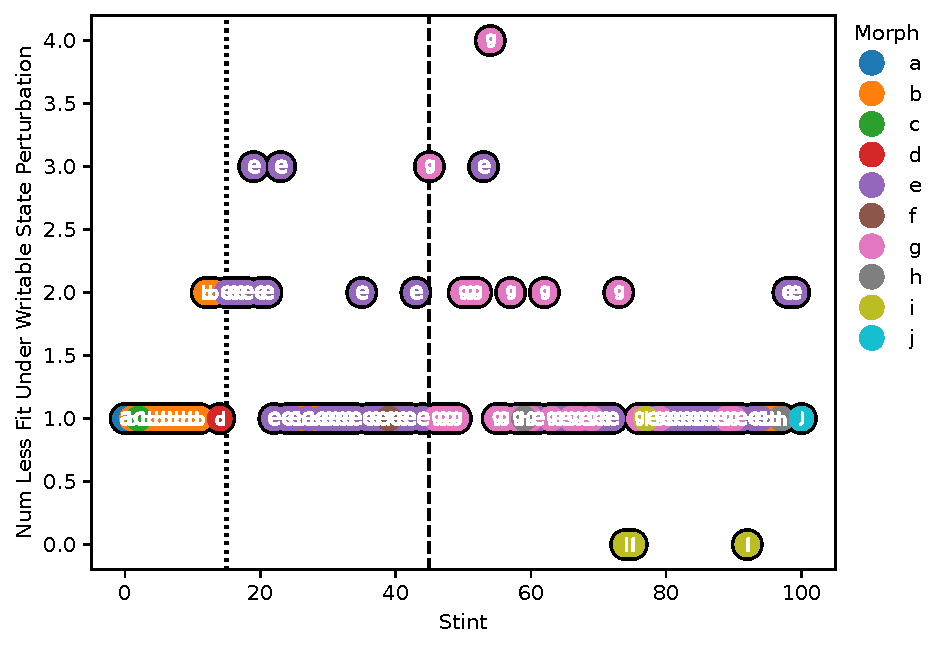
\includegraphics[width=\linewidth]{{plots/writable_interface_complexity/bucket=prq49+cat=morph+endeavor=16+transform=filter-Series-16005+viz=letterscatter-vline+x=stint+y=num-less-fit-under-writable-state-perturbation+ext=}}

\caption{Writable state interface complexity, the number of output states that contribute to fitness. See Supplementary Figure \ref{fig:writable_perturbation} for detail on the writable states that contribute to fitness.}
\label{fig:interface_complexity:writable_interface_complexity}

\end{subfigure}%

\caption{ Interface complexity estimates. Color coding and letters correspond to qualitative morph codes described in Table \ref{tab:morph_descriptions}.
Dotted vertical line denotes emergence of morph $e$.
Dashed vertical line denotes emergence of morph $g$.}
\label{fig:interface_complexity}
\end{figure*}


Figure \ref{fig:interface_complexity} summarizes cardinal interface complexity, as well as its constituent components, for specimens drawn from across the case study's evolutionary history.

%todo: not a sentence
Notably, cardinal interface complexity more than doubles from 6 interactions to 17 interactions coincident with the emergence of morph $e$ (Figure \ref{fig:interface_complexity:cardinal_interface_complexity}).
This is due to simultaneous increases in extrospective state sensing (2 to 9 states; Figure \ref{fig:interface_complexity:extrospective_interface_complexity}), introspective state sensing (1 to 4 states; Figure \ref{fig:interface_complexity:introspective_interface_complexity}), and writable state usage (1 to 2 states; Figure \ref{fig:interface_complexity:writable_interface_complexity}).

The emergence of morph $g$ coincided with an increase in writable state interface complexity from 1 to 3 as shown in Figure \ref{fig:interface_complexity:writable_interface_complexity}.
However, morph $g$ was not associated with other changes in other aspects of cardinal interface complexity.
The greatest observed cardinal interface complexity was 22 interactions at stints 54 and 67.